\subsection{Versionskontrolle mit Git}
\subsubsection{Allgemeines}
Die Versionskontrolle oder Quellcodekontrolle ermöglicht es, Änderungen an
Softwarecode zu verfolgen. Die Verfolgung aller Änderungen erlaubt bei Bedarf
die Wiederherstellung eines früheren Datenstands. \parencite{git-allgemein}

Versionskontrollsysteme, wie Git, speichern jede Änderung am Code in speziellen
Git-Datenbank-Dateien. Programmierer können dadurch in ihren Teams genau
analysieren, wer welche Zeile wann geändert oder neu eingesetzt hat.

Durch Git können mehrere Entwickler an demselben Projekt bzw. Repository
arbeiten und sogar dieselben Dateien gleichzeitig ändern. Oftmals entstehen
Konflikte, wenn zwei oder mehr Personen an derselben Datei arbeiten. Git enthält
hierfür Prozesse, um solche Konflikte sauber lösen zu können. Beim
Zusammenführen der beiden Zustände kann man entscheiden, welche Zeile man aus
welcher Änderung übernimmt.

Git bietet durch die Speicherung jeder Änderung nicht nur den Vorteil
gemeinsamen Arbeitens, sondern auch eine Art \glqq Backup\grqq{}. Durch den
genauen Verlauf des Quellcodes, können Fehlerursachen schneller analysiert,
gefunden und verifiziert werden. Um die einzelnen Snap\-shots bzw.
Schnappschüsse des aktuellen Standes zu markieren, gibt es in Git die
sogenannten Commits.

\newpage

Die folgenden Begriffsklärungen und Anleitungen rund um das
Versionskontrollsystem Git sind wichtig, um den Rest der Arbeit besser verstehen
zu können.

\subsubsection{Repositorys und Commits}
Das Git-Repository ist der Kern des Projekts und umfasst alle Dateien, die von
Git überwacht werden sollen. Es ist sozusagen das Projekt, an dem die Entwickler
arbeiten. Um ein Repository anzulegen, braucht es nur einen Ordner, in dem man
in der Konsole folgenden Befehl ausführt:
\begin{lstlisting}[style=Bash]
$ git init
\end{lstlisting}
Daraufhin wird in diesem Verzeichnis ein neuer \texttt{.git}-Ordner erstellt,
welcher alle Informationen über das gerade erstellte Repository enthält. Sobald
man nun beispielsweise eine neue Textdatei anlegt, wird der Erstellvorgang im
\texttt{.git}-Ordner getrackt.

Git arbeitet mit Snapshots, die manuell angelegt werden müssen. Wenn der
Entwickler nun täglich einen Absatz in die Textdatei schreibt, gibt es hierfür
keine Historie. Git weiß nur, dass im ersten Snapshot keine Datei vorhanden war
und nun eine Datei mit gefülltem Text vorliegt.

Um einen Verlauf der Erstellung zu speichern, muss der Entwickler sogenannte
Commits mit aktuellen Zeitstempeln erstellen. Wann die Commits jeweils erstellt
werden, ist dem Entwickler selbst überlassen. In der Regel werden Commits immer
nach dem Erreichen eines Meilensteins erstellt. In diesem Fall wäre ein
täglicher Meilenstein das Abschließen eines neuen Absatzes in der Textdatei.
Zuerst können alle geänderten Dateien in der Konsole mit folgendem Befehl
abgerufen werden:

\begin{lstlisting}[style=Bash]
$ git status
On branch main

No commits yet

Untracked files:
(use "git add <file>..." to include in what will be committed)
    hallo-welt.txt

nothing added to commit but untracked files present (use "git add" to track)
\end{lstlisting}

\newpage

Wie die Ausgabe auf der vorherigen Seite bereits verrät, wurde bisher noch kein
Commit angelegt. Außerdem zeigt sie, dass die Datei \texttt{hallo-welt.txt}
angelegt wurde, bisher jedoch nicht getrackt wird. Nun kann der Entwickler die
Änderung tracken, indem er folgenden Befehl ausführt:

\begin{lstlisting}[style=Bash]
$ git add hallo-welt.txt
\end{lstlisting}

Durch den Befehl \code{git add .} wäre es zudem möglich mit einem Kommando alle
\emph{untracked} (nicht verfolgten) Änderungen verschiedener Dateien in den
neuen Commit hinzuzufügen. Schließlich weiß Git jetzt, welche Änderungen
committet werden sollen. Mit dem Befehl

% TODO: hier weiter machen
\begin{lstlisting}[style=Bash]
$ git commit -m "Neue Hallo Welt Datei angelegt"
\end{lstlisting}

\noindent
wird ein Commit mit der Nachricht \glqq Neue Hallo Welt Datei\grqq{} angelegt.
Dies ist nun ein neuer Snapshot, welcher in der Commit-Historie gespeichert
wird. Sollte der Programmierer die Datei erneut verändern, kann er die neuen
Änderungen wieder tracken und schließlich committen. An diesem Punkt könnte er
jedoch jederzeit zu dem alten, bereits committeten Zustand zurückkehren.

Damit ein Repository im Internet verfügbar ist, benötigt man einen Server mit
einer Kopie des lokalen Repositorys. Diese Repositorys nennt man auch
Remote-Repositorys. Der bekannteste Dienstleister für die Speicherung
von Remote-Repositorys ist GitHub. Der Vorteil von einer Online-Version des
eigenen Repositorys ist, dass andere Entwickler das Projekt klonen und
anschließend daran mitarbeiten können. Nach dem Klonvorgang haben diese Personen
ebenfalls eine lokale Kopie des Repositorys auf ihrem Endgerät. Um nun einen
lokalen Commit online verfügbar zu machen, muss dieser \emph{gepusht} werden.

Zuerst muss über folgenden Befehl geprüft werden, ob im lokalen Repository das
richtige Remote-Repository referenziert wird:

\begin{lstlisting}[style=Bash]
$ git remote -v
origin	https://github.com/user/repository-name (fetch)
origin	https://github.com/user/repository-name (push)
\end{lstlisting}

Sollten die Adressen zum richtigen Online-Repository verweisen, kann mit
folgendem Befehl ein Commit hochgeladen werden:

\begin{lstlisting}[style=Bash]
$ git push
\end{lstlisting}

\newpage

Um mögliche Änderungen durch andere Mitarbeitende in das eigene lokale
Repository zu laden, benötigt man wiederum einen sogenannten \emph{Pull}:

\begin{lstlisting}[style=Bash]
$ git pull
\end{lstlisting}

Der Git-Workflow umfasst noch viele weitere Befehle und kann für Unerfahrene
schnell sehr kompliziert werden. Aus diesem Grund enthalten die meisten gängigen
Entwicklungsumgebungen grafische Oberflächen für die Verwendung von Git. So
benötigt der Entwickler weder die Kommandozeile noch tieferes Fachwissen über
die genaue Verwendung bzw. Syntax der Befehle.

\subsubsection{Branches}
Git bietet neben der Kontrolle und Verfolgung von Commits und Änderungen auch
die Möglichkeit echt parallel zu arbeiten. In einem großen Softwareprojekt sind
zur Laufzeit auftretende Fehler in der Regel unumgänglich. Um keine Kunden zu
verlieren, müssen einige dieser Fehler gegebenenfalls schnellstmöglich behoben
werden.

In diesem beispielhaften Fall, dass in einer Software ein gravierender Fehler
auftritt, sollte möglichst schnell ein Update mit einer Lösung ausgearbeitet
werden. Es kann jedoch sein, dass ein Teil des Entwicklungsteams gerade an einem
sehr großen neuen Feature arbeitet, welches nicht unvollständig veröffentlicht
werden darf. Es muss also eine Lösung gefunden werden, damit eine neue Version
mit dem behobenen Fehler veröffentlicht werden kann, ohne, dass die Arbeit an
dem neuen Feature gestört oder rückgängig gemacht werden muss. Git stellt mit
dem Konzept von Branches eine Lösung für dieses Problem dar.

\begin{figure}[h]
    \centering
    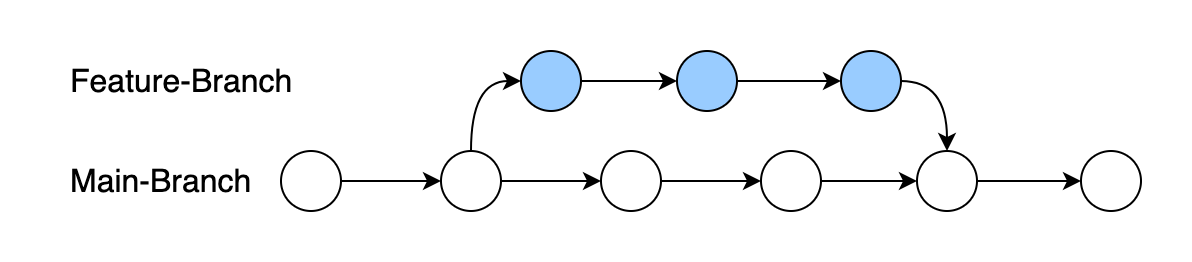
\includegraphics[width=\textwidth]{git-branch}
    \caption{Git: Branches}
    \bildquelle{Eigene Darstellung}
    \label{fig:git-branch}
\end{figure}

Branches (Äste) teilen den linearen Entwicklungsablauf in mehrere parallele
Zustände. Standardmäßig arbeitet man bei Git auf dem \texttt{Main}-Branch -- Der
Hauptzweig sozusagen (siehe \autoref{fig:git-branch}, der weiße Strang).
Die weißen Kugeln stellen in der Grafik jeweils einzelne Commits dar. Sobald ein
neues Feature entwickelt wird, möchte der zuständige Programmierer nicht, dass
sich während der Entwicklung der Funktion etwas am restlichen Code ändert. Aus
diesem Grund eröffnet der Feature-Programmierer, wie in \autoref{fig:git-branch}
ersichtlich, einen neuen Branch auf den aktuellen Commit des Hauptzweigs (blauer
Zweig). Wenn sich der Hauptzweig nun durch Überarbeitungen von anderen Kollegen
ändert, merkt der Feature-Programmierer nichts davon, weil er sich auf einem
anderen Ast (Branch) befindet und dabei seine ganz eigene Kopie des Projekts
bearbeitet. Sobald er mit dem Feature fertig ist, kann er seinen Branch mit dem
\texttt{Main}-Branch wieder zusammenführen. Falls sich in der Zwischenzeit die
Dateien und Zeilen, die auch er bearbeitet hat, geändert haben, müssen die
Konflikte in aller Regel manuell gelöst werden. Sollten nicht dieselben Zeilen
bearbeitet worden sein, löst Git die Konflikte selbst und führt die zwei
Zustände automatisch zusammen.

Eine bekannte Konvention unter Programmierern ist es, dass der
\texttt{Main}-Branch immer eine lauffähige Version der Software hält. Es darf
nie ein nicht-kompilierbarer oder unfertiger Stand auf dem Hauptzweig landen.
So stellt man sicher, dass neue abzweigende Branches immer auf einer
lauffähigen Basis aufbauen. \parencite{git-branches}

\begin{figure}[H]
    \centering
    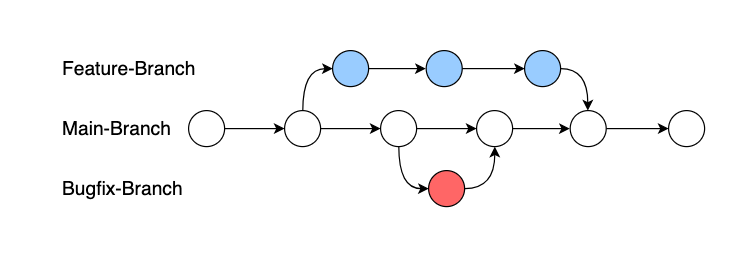
\includegraphics[width=\textwidth]{git-branch-fehler}
    \caption{Git: Branches (Bugfix-Branch)}
    \bildquelle{Eigene Darstellung}
    \label{fig:git-branch-fehler}
\end{figure}

Wie in \autoref{fig:git-branch-fehler} zu erkennen, werden auch Fehlerbehebungen
(Bugfixes) meist in einem anderen Branch behandelt. Nun lässt sich auch die
anfangs erläuterte Problemstellung leicht erklären. Wenn ein gravierender
Softwarefehler auftritt, kann das Team ausgehend vom lauffähigen
\texttt{Main}-Branch einen neuen Zweig zur Fehlerbehebung eröffnen (siehe
\autoref{fig:git-branch-fehler}, roter Kreis). Auf diesem Zweig können sie
unabhängig von der Entwicklung eines neuen Features den Fehler beheben, mit dem
Hauptzweig zusammenführen und das Update veröffentlichen. Wenn das Feature
fertig ist, wird der \texttt{Feature}-Branch mit dem Hauptzweig zusammengeführt
und der Fehler auch darin automatisch behoben. Sollte der Fehler so gravierend
sein, dass er die Entwicklung des \texttt{Feature}-Branches behindert, kann man 
jederzeit den nun fehlerfreien \texttt{Main}-Branch in den
\texttt{Feature}-Branch mergen und den \texttt{Feature}-Branch somit wieder auf
den aktuellen Stand bringen. Mergen heißt hier nichts anderes als das
Zusammenführen zweier Codebasen. Dies ist auch sinnvoll, wenn die Entwicklung
eines Features einen längeren Zeitraum beansprucht. Ansonsten geht man die
Gefahr ein, dass sich der Hauptzweig bei der Zusammenführung so sehr verändert
hat, dass er sich zu sehr vom \texttt{Feature}-Zweig unterscheidet und ein Merge
sehr viel manuelle Arbeit erfordern würde.
